\chapter{Computing with particles}
\label{app:computing-with-particles}

The particle filter allows us to approximate any distribution by using a sample of \emph{particles}, $x\vi$, with weights $w\vi$. There are many advantages of the particle filter, but one is that producing summary statistics is very simple. The only real disadvantage is that it is a computationally demanding process. In this appendix, we briefly descibe the theory behind using the particle filter to estimate a distribution, as well as give details on its computational demands.


\section{The Dirac measure}
\label{app:dirac-delta-measure}

In \cref{sec:recursive-bayes,cha:vehicle_model} we described the particle filter implementation, and noted that we can use the Dirac measure, $\dirac$, to approximate the distribution. We will not got into the theoretical aspects of the function, except to state the following property \citep{cn}:
\begin{equation}
\label{eq:dirac_property}
\int_X f(x) \dirac_y(x)\dx = f(y).
\end{equation}

Let $x$ be an unknown quantity for which we have a sample of $N$ particles $\{x\vi\}_{i=1}^N$ with associated weights $\{w\vi\}_{i=1}^N$. The Dirac delta measure is used to approximate the distribution of $x$ \citep{cn}:
\begin{equation}
\label{eq:dirac_dist}
p(x) \approx \sum_{i=1}^N w\vi \dirac_{x\vi}(x)
\end{equation}


Using \cref{eq:dirac_property,eq:dirac_dist} we can now compute, for example, the mean, $f(x) = x$,
\begin{equation}
\label{eq:dirac_mean}
\begin{split}
\bar x &= \int_X x p(x) \dx \\
&= \int_X x \sum_{i=1}^N w\vi \dirac_{x\vi}(x) \dx \\
&= \sum_{i=1}^N w\vi \int_X x \dirac_{x\vi}(x) \dx \\
&= \sum_{i=1}^N w\vi x\vi.
\end{split}
\end{equation}




\section{Resampling}
\label{app:particle-resampling}

Part of the particle filter update step is to, when required, resample the particles according to their weights. This involves generating random numbers to determine which particles to include in the sample, replacing the vector of particle states with the new sample. The latter is straightforward: we simply copy the sampled particles into a new vector and, once finished, replace the original vector with the new one.


We will now describe unweighted resampling first before discussing weighted. Given a sample of size $N$, we use a \gls{rng} to obtain uniform numbers $u \in (0, 1)$. Since each particle has equal weight, we multiply $u$ by $N$ and round down (using the \emph{floor} function), so get
\begin{equation}
j = \lfloor uN \rfloor.
\end{equation}
Thus, we have sampled particle $j$.


When the particles are weighted, however, we cannot simply use $uN$. For example, here we have five particles, where each is represented by a rectangle whose width is equal to the particle's weight (the total weight is unity), as shown in \cref{fig:app_weighted_resampling}.
\begin{knitrout}\small
\definecolor{shadecolor}{rgb}{0.969, 0.969, 0.969}\color{fgcolor}\begin{figure}[h]

{\centering 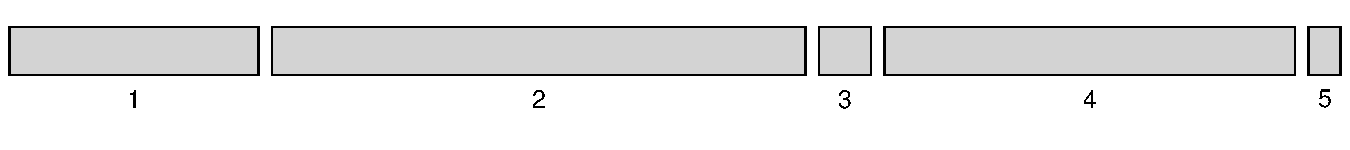
\includegraphics[width=0.8\textwidth]{figure/app_weighted_resampling-1} 

}

\caption[Particle weights]{Particle weights.}\label{fig:app_weighted_resampling}
\end{figure}


\end{knitrout}

As before, we use a \gls{rng} to obtain a uniform random number $u$; to map the number to a particle, we compute \emph{cumulative weights} and find the maximum weight less than $u$:
\begin{equation}
j : \sum_{i=1}^j w\vi[j] \leq u.
\end{equation}




\section{Summary statistics}
\label{app:particle-summaries}

Another core part of the program is computing of summary statistics, for example the mean and variance. However, these are easily computed using \verb+std::accumulate+, for example, a vehicle's mean speed is obtained by:
\begin{lstlisting}
double mean = std::accumulate (
    x.begin (), x.end (),
    // initial value
    0.,
    // lambda function, where 'a' is the current value
    [](double a, Particle& p) {
        return a + p.get_weight () * p.get_speed ();
    }
);
\end{lstlisting}
Similarly, the variance can be calculated by passing a reference to the value of \verb+mean+ to the lambda function (within \verb+[]+), which becomes
\begin{lstlisting}
[&mean](double a, Particle& p) {
    return a + p.get_weight () * pow (p.get_speed () - mean, 2.);
}
\end{lstlisting}

More complicated, however, is estimation of \emph{quantiles}, since this requires sorting the vector of particles in order of the desired value. In the above example, to get the median speed, we need to first sort the particles by speed (slowest to fastest) and then sum their weights, in order, until the sum surpasses 0.5: the speed of the particle that does so is the median speed.
\begin{lstlisting}
std::sort (x.begin (), x.end (),
    (Particle& p1, Particle& p2)
    {
        return p1.get_speed () < p2.get_speed ();
    }
);
double wt = 0.;
int i = 0;
while (wt < 0.5) wt += x.at (i++).get_weight ();
double median = x.at (i).get_speed ();
\end{lstlisting}

The issue here is the first step, sorting, which has computational complexity of $\mathcal{O}(N\log N)$\footnote{as described by the documentation page for \verb+std::sort+, \url{https://en.cppreference.com/w/cpp/algorithm/sort}}. If we wish to estimate the median distance and the median speed, we need to sort the particles \emph{twice}. In \cref{cha:etas}, we used multiple quantiles for each stop: this requires sorting each vehicle's particles once for each upcoming stop. However, since we use a subsample to compute \glspl{eta} ($N^\star$), the complexity is significantly smaller, $\mathcal{O}(N^\star\log N^\star)$; if we attempted to use all $N$ particles (in the simulation used in \cref{cha:prediction}, we used $N=10000$) the application would have taken far longer.
